\documentclass[12pt, a4paper, ngerman]{article}

\usepackage{geometry}
\geometry{outer=2.5cm,inner=2.5cm,top=3cm,bottom=2cm,headsep=1cm,footskip=2cm}

\usepackage[utf8]{inputenc}
\usepackage[T1]{fontenc}
\usepackage[ngerman]{babel}
\usepackage{lmodern}
\usepackage{hyphenat}
\hyphenation{Mathe-matik wieder-gewinnen}

\usepackage{graphicx}
\usepackage{hyperref}
\usepackage[parfill]{parskip}
\usepackage{enumitem}

\usepackage{fancyhdr}
\pagestyle{fancy}
\fancyhf{}
\lhead{\textsc{Mobile Computing - WS21/22}}
\rhead{\textsc{Ekrem Emre}}	

\let\svthefootnote\thefootnote
\renewcommand{\headrulewidth}{0.5pt}

\begin{document}

\section*{Rosalyn Foster}
\subsection*{Persona}

\begin{figure}[htp]
\centering
  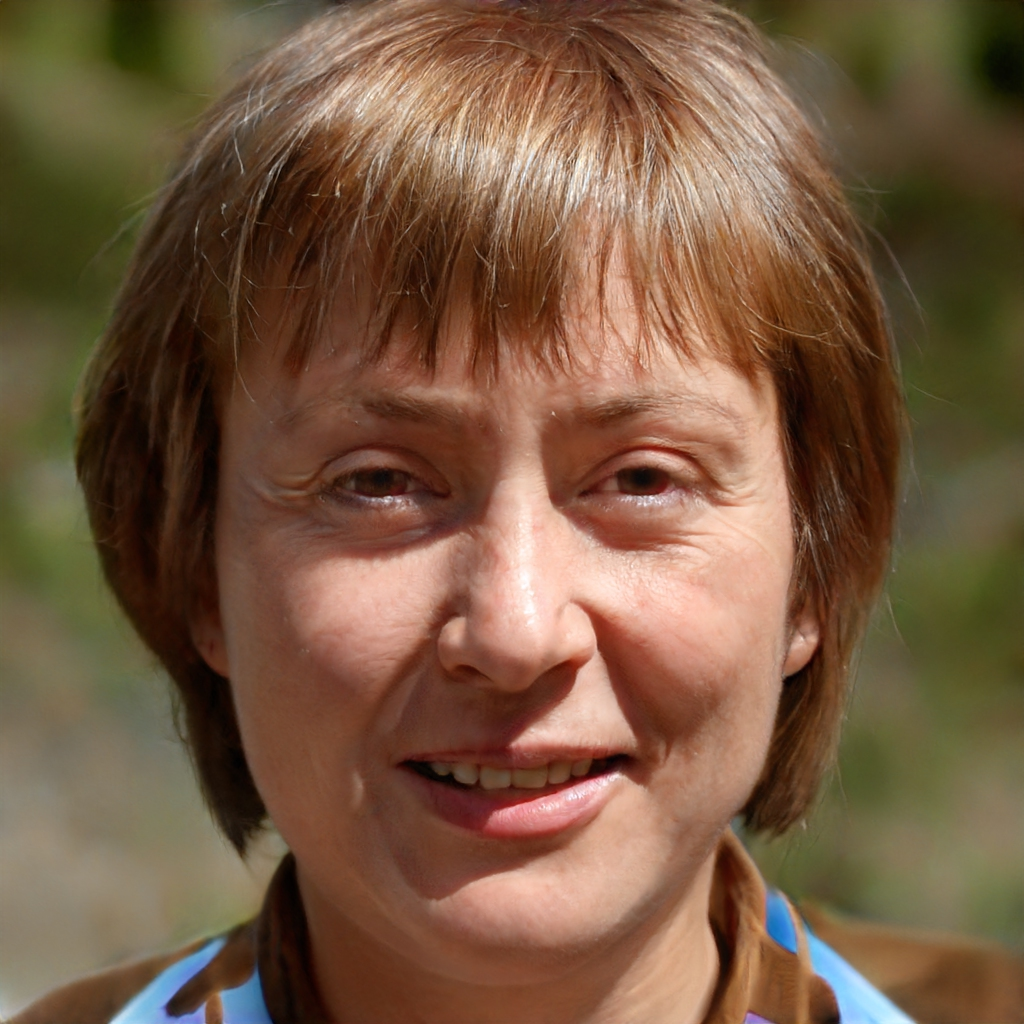
\includegraphics[height=0.5\textwidth]{images/persona01.jpg}
\end{figure}
\let\thefootnote\relax\footnotetext{Image source: \url{https://thispersondoesnotexist.com/}}

\textbf{Name:} Rosalyn Foster \\
\textbf{Age:} 68 \\
\textbf{Marital status:} Married \\
\textbf{Occupation:} Retiree  \\
\textbf{Computer skills:} minimal

\subsubsection*{Key characteristics}

\begin{itemize}[noitemsep]
	\item Retiree, former tailor.
	\item Because of her advanced age, she got forgetful.
	\item Is regularly taking different medication, which needs she needs to be reminded of.
	\item Is concerned about her health, because she just became a grandparent and wants to spent as much time as possible with her grandchildren.
\end{itemize}

\subsubsection*{Goals}

\begin{itemize}[noitemsep]
	\item Be healthy.
	\item Remember taking her medication regularly.
\end{itemize}

\subsection*{User Stories}

As an older person, Rosalyn wants to be reminded to take her medicine, because she forgets them and wants to get healthy.

%Rosalyn just got a new prescription from her doctor. The medicine is a pill, which she needs to to take every day at lunchtime.
%After her prescribed medicine had unwanted side effects, the doctor told her discontinue the medicine and gave her a new prescription.

\newpage

\section*{Christian Metz}
\subsection*{Persona}

\begin{figure}[htp]
\centering
  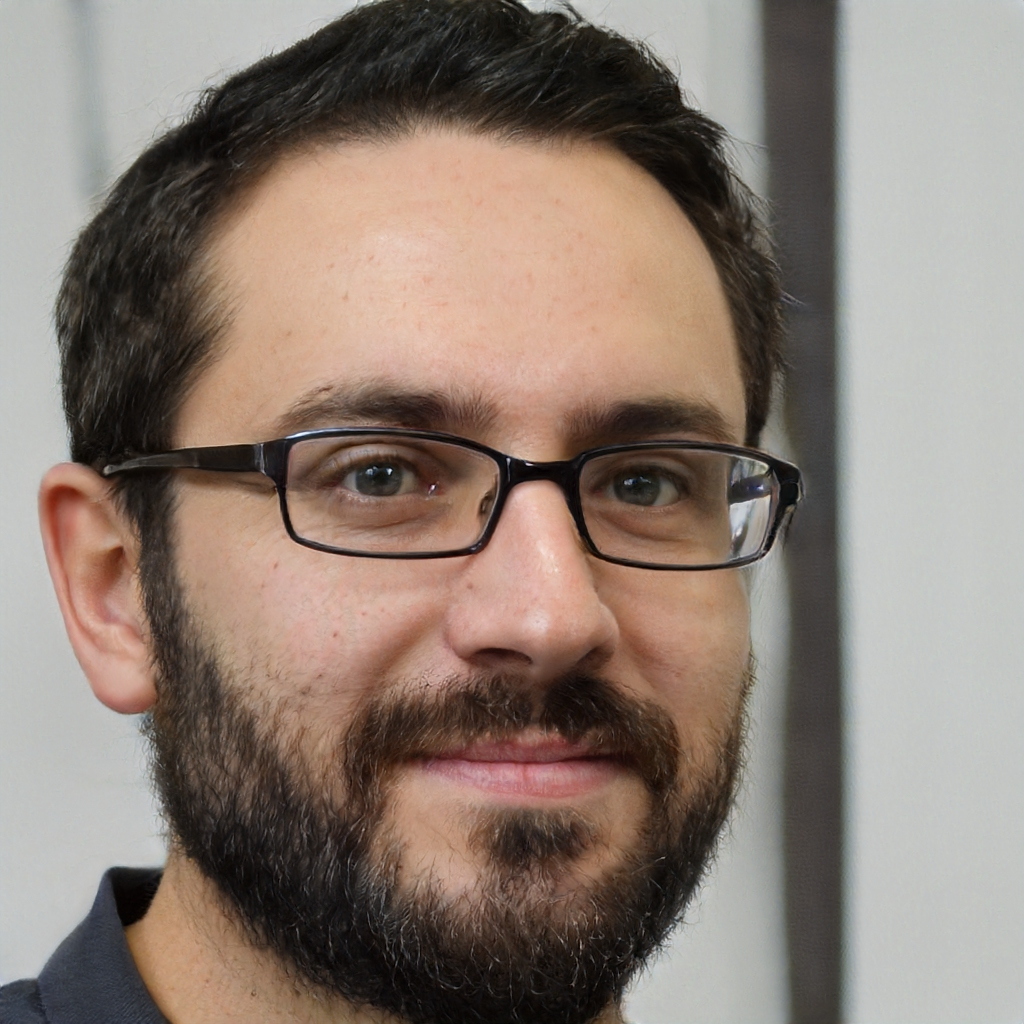
\includegraphics[height=0.5\textwidth]{images/persona02.jpg}
\end{figure}
\let\thefootnote\relax\footnotetext{Image source: \url{https://thispersondoesnotexist.com/}}

\textbf{Name:} Christian Metz \\
\textbf{Age:} 32 \\
\textbf{Marital status:} Engaged \\
\textbf{Occupation:} Physiotherapist \\
\textbf{Computer skills:} 
\subsubsection*{Key characteristics}

\begin{itemize}[noitemsep]
	\item Working as a physiotherapist and doing a lot of sports, therefore is very healthy.
	\item He's a member in several sport clubs and a volunteer in the local animal shelter.
	\item His schedule is always pretty full and he's always on the go.
	\item He wants to increase his health by taking some vitamins, because he suspects he has some deficiencies.
\end{itemize}

\subsubsection*{Goals}

\begin{itemize}[noitemsep]
	\item Be reminded, to take his vitamins.
\end{itemize}


\subsection*{User Stories}

As a healthy person, Christian wants to be reminded to take his vitamins, because he's busy all day and not thinking of it and wants to stay healthy.

\end{document}
